\chapter{Vymezení legacy aplikace}
V této kapitole bude nadefinován termín legacy aplikace. První část kapitoly bude věnována vymezení legacy aplikace a bude představena její architektura. V druhé části kapitoly jsou popsány problémy, které vznikly během potřeby udržovat tento typ aplikací v provozu. 

\section{Definice}
Termín legacy aplikace není jednoduché nadefinovat. Podle zdrojů \cite{legacy1} a \cite{legacy2} bývá vykládán a používán v mnoha různých kontextech. Obecně se dá říci, že se jedná o aplikaci, která je postavena na zastaralém hardwaru a provozována na neaktuálních operačních systémech. Tyto systémy jsou v současné době stále používány a udržovány v běhu na původním hardwaru. Problémem je často značná složitost aplikace a nedostatečná či nepřesná dokumentace. Některé legacy aplikace běží na mainframech. Dále se jedná o aplikace se zastaralou architekturou či napsané ve starých programovacích jazycích. Hovoříme zejména o rozlehlé monolitické aplikace, které jsou velmi těžko spravovatelné. Důvodem, proč tyto staré systémy bývají udržovány, je jejich kritická funkcionalita. Například v organizaci NASA jsou stále systémy tohoto typu využívány pro vesmírný výzkum \cite{NASA_legacy}. NASA ve svém výzkumu používá i některé technologie a systémy, které byly vytvořeny během 70. let minulého století.

\section{Monolitická architektura}
Co se týká architektury, je velmi těžké stanovit jeden typ, jelikož mnoho legacy aplikací je postaveno na rozdílných architekturách. Často bývá monolitická architektura označována jako legacy. Obecně lze říci, že monolitická aplikace je složena z jednoho velkého balíku zdrojového kódu, který obsahuje všechny komponenty. Implementace monolitické architektury bývá zprvu jednoduchá a lépe se s ní pracuje z důvodu sdíleného kódu. S přidáváním komponent začne být aplikace složitější z důvodu soudržnosti zdrojového kódu. Například refaktorování zdrojového kódu může negativně ovlivnit aplikaci. Dalším problematickým faktorem je testování aplikace. Aplikace je jeden logický celek, kterému je nutné přizpůsobit funkční testy, které bývají mnohem složitější a časově náročnější než testování jednotlivých komponent aplikace \cite{legacy_testing}. Největším problémem monolitické aplikace je její nasazení a provoz. Pro nasazení nových verzí aplikace je nutné nasazovat aplikaci jako celek. Proces aktualizace často vyžaduje velké množství skriptu a manuálních procesů, které je velmi obtížné zautomatizovat. Stejný problém je se škálováním aplikace, protože není možné škálovat jednotlivé části aplikace ve více kopiích. Naopak je nutno spouštět celou repliku aplikace jako celek. Tato skutečnost vede ke plýtvání se zdroji. Při naškálovaných zdrojích bude server s aplikací konzumovat větší množství zdrojů, které nebudou plně využity. Jak již bylo zmíněno, tato architektura má řadu nevýhod. I přes tuto skutečnost bývá tento typ architektury používán především u menších aplikací, které nepotřebují škálovat a neobsahují složitou business logiku.

\begin{figure}[H]
\begin{centering}
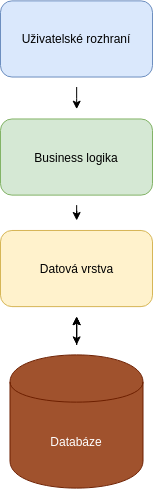
\includegraphics[width=0.2\textwidth]{img/monolit.png}
\par\end{centering}
\caption{Schéma monolitické architektury, zdroj: vlastní tvorba} \label{fig:monolit}
\end{figure}

Při porovnání použití architektury mikroslužeb a monolitické architektury se nedá jednoznačně stanovit, která architektura je složitější. Co se týká granularity a velikosti mikroslužeb, bývají tyto díky svému dělení mnohem rozsáhlejší než monolitická architektura. Jednotlivé služby však bývají od sebe izolovány, a to umožňuje jednotlivým komponentám nezávislost, což je výhodné především při testování a nasazování nových verzí. Tato výhoda se zpravidla projevuje u instalací, kdy není potřeba celou aplikaci znovu instalovat, jak tomu bývá u monolitické architektury. Z pohledu provozu monolitické aplikace bývají všechny funkce zabaleny do jednoho procesu, který poté spouští celou aplikaci. Problém jednoho procesu se projeví u škálování, protože oproti mikroslužbám není možné spustit více replik části aplikace a je nutné aplikaci duplikovat celou. Porovnání architektur je v tabulce číslo \ref{tbl:mono_ms}.

\begin{table}[H]
\begin{center}
\caption{Porovnání monolitické architektury a mikroslužeb} 
\label{tbl:mono_ms}
\begin{tabular}{|p{40mm}|p{50mm}|p{50mm}|}
\hline
  ~   & Monolitická architektura & Mikroslužby \\    \hline
Zdrojový kód: &  Jednotný kód &  Kód je rozdělen do více na sobě nezávislých celků  \\    \hline
Programovací jazyky: &  Aplikace je napsaná v jednom programovacím jazyce. & Každá služba je oddělená aplikace, která může být napsána v různých programovacích jazycích. Nutná je pouze standardizace komunikace mezi službami. \\    \hline
Granularita kódu: & Vysoká & Nízká  \\    \hline
Škálování: & Aplikaci je nutno škálovat jako celek je nezbytné škálovat i služby, které nebudou plně využívány. & Lze škálovat pouze jednotlivé části aplikace nezávisle na sobě. \\    \hline

\end{tabular}
\end{center}
\end{table}

\section{Problémy}
V následující části kapitoly jsou popsány problémy legacy aplikací. U jednotlivých problémů je  naznačeno, jak je lze vyřešit pomocí současných řešení a technologií.

\subsection{Metodologie vývoje}
Obtížnou práci s legacy aplikacemi může způsobit kromě architektury i model vývoje softwaru, který byl použit. V těchto aplikacích probíhalo řízení projektu pomocí tzv. vodopádového vývoje (waterfall). Tento model byl nadefinován Winstonem W. Roycem, který ho zveřejnil ve svém článku „Managing the Development of Large Software System“. Již v roce 1970 byl samotným autorem tento model označen jako příklad nefungujícího modelu. Model je postaven na základním principu sedmi vrstev složených ze specifikace požadavků, návrhu, implementace, integrace, testování a ladění (validace), instalace a údržba. Mezi jednotlivými vrstvami nelze přecházet, pokud nejsou jednotlivé úkoly v dané vrstvě dokončeny. Mezi jednotlivými vrstvami se lze pohybovat pouze vpřed. Model klade důraz především na plánování, a proto je nutné mít všechny funkční požadavky připravené ještě před samotnou tvorbou aplikace. Nevýhodou vodopádového přístupu je jeho malá flexibilita a pomalý vývoj, protože je nutné mít jednotlivé kroky předem naplánované z důvodu, že později už není prostor na změny. Aby byl model flexibilnější, začaly ho jednotlivé firmy upravovat dle svých potřeb. I přes veškeré modifikace tento model vývoje nebyl úspěšný natolik, aby mohl být v současnosti masově využíván. V dnešní době je potřeba rychlého vývoje aplikací. Nové verze nástrojů a technologií vychází každý týden, a je tedy nutné tuto skutečnost zohlednit již při vývoji aplikace samotné. I přes obrovskou jednoduchost vodopádového přístupu je model jen zřídka využíván v praxi. Slouží převážné k teoretické výuce softwarového inženýrství nebo je použit pouze ve velkých organizacích, které mají předem určený rozpis požadavků a kroků.(NASA \cite{NASA_legacy}, vládní projekty).

Přesným opakem vodopádového přístupu jsou agilní metodiky, které jsou založeny na iterativním přístupu k problému. Tento způsob plánování byl vytvořen především pro potřeby rychlého vývoje softwaru. V dnešní době se agilní přístup využívá také v dalších oborech a odvětvích, jako je například marketing. Stavební kámen agilní metodiky je manifest agilního programování \cite{agilni_manifest}, který byl navržen a vytvořen v roce 2001 na setkání odborníků softwarového plánování. Největším rozdílem mezi vodopádovým a agilním přístupem je čas reakce na změnu požadavků. Pokud se zákazník rozhodne něco změnit v průběhu implementace v agilním přístupu, je velmi jednoduché na změnu reagovat, lze ji zahrnout do nadcházející iterace. Agilní metodika v dnešní době slouží i jako odrazový můstek pro tvorbu dalších přístupů ve vývoji. Jedná se o modely jako XP, Scrum, FDD, TDD. Jedním z přístupů, který za posledních pár let vzrostl na popularitě, je Scrum. Scrum systém je založen na iteračních cyklech, které se nazývají sprint. Sprinty se opakují v pevně daném časovém období, zpravidla čtrnáctidenních cyklech. Na začátku sprintu jsou vždy vymezeny problémy, které se budou ve sprintu řešit. Pro každý problém je pevně určen vlastník problému, který obvykle zastupuje v procesu roli zákazníka, ale nezasahuje do vývojového procesu. Poté jsou jednotlivé problémy rozděleny mezi vývojový tým, který je vždy zodpovědný za vyřešení daného úkolu nebo přidání nové funkcionality. Na konci sprintu by měla být nová funkcionalita implementovaná ve funkční podobě. Vývojové týmy bývají složeny z menšího počtu osob, cca do deseti vývojářů. V menším počtu jsou vývojáři schopni efektivněji spolupracovat a pracovat flexibilněji. Jednotlivé vývojové týmy jsou víceúčelové a spolupracují od analýzy přes vývoj až po dokumentaci. Poslední entita, která figuruje v scrum procesu, je tzv. scrum master, který hledá překážky ve vývoji a pracuje na jejich odstranění. Zároveň kontroluje, zda se dodržuje scrum proces a zda vše probíhá tak, jak bylo naplánováno. Podobně jako u vodopádového přístupu, tak i u scrumu některé firmy, které koncept přebírají, jej upravují podle svých potřeb. Například švédská firma Spotify si vystavěla svůj Squad framework \cite{squad_framework}, který celý scrum proces mění a přidává další koncepty. Největší výhodou scrumu a agilního vývoje obecně je obrovská rychlost vývoje a schopnost doručovat zákazníkům nové vlastnosti rychleji.

\subsection{Hardware}
První problém, který souvisí s provozem legacy aplikací, je hardware. Zdrojový kód legacy aplikace je často přizpůsoben k provozu na konkrétní hardwarové platformě. Dříve byly tyto platformy spravovány pouze jediným vendorem, což vedlo k uzamčení se na jednoho výrobce. Pokud pochází hardware od specializovaného vendora, je velmi nákladné tento hardware spravovat. Důvodem je především dostupnost uživatelské podpory ze strany poskytovatele hardwaru. Pokud je podpora pro hardware dostupná, je zpravidla velmi drahá.

Problémy se závislostí na vendoru lze vyřešit pomocí komoditního hardwaru, který je složen z komponent  třetích stran. Tyto komponenty jsou velmi jednoduché na výměnu. Posléze pak není složité vyměnit celý server za jiný. Tento typ hardwaru je o proti specializovanému hardwaru výrazně levnější. 

\subsection{Udržování aplikace}
V této části budou uvedeny problémy spojené s udržováním legacy aplikací. Pokud je třeba aplikaci rozšířit nebo upravit, je nutné aplikaci dodatečně doladit. Proto je u starých aplikací složených z většího počtu komponent nezbytné udržovat aktuální dokumentaci, aby se do dodatečného vývoje aplikace mohli zapojit i programátoři, kteří aplikaci nevyvíjeli. Důležitým faktorem pro udržování a rozšiřování jsou aktuální testy aplikace, ty bývají ve velké části případů vývoje zanedbávány \cite{legacy_testy}. Ať už se jedná o funkční či unit testy, je nutné mít alespoň základní sadu scénářů, se kterou lze vyvíjenou aplikaci vyzkoušet. Další komplikací, která vede k neefektivní práci vývojářů, jsou také vývojová prostředí. Velké množství komponent a tříd vede ke zpomalení vývojových nástrojů (IDE).

\subsection{Aktualizace a CI/CD}
Dalším problémem může být doručování aktualizací a opravných záplat do již běžící aplikace. Staré aplikace byly většinou navrhovány pro jeden způsob užití. Byly nasazeny do produkčního prostředí a, pokud byly funkční, nebylo nutno se o ně starat. Podle zdroje \cite{legacy_years} byly některé legacy systémy v provozu i několik desítek let. I když by daná aplikace nevyžadovala žádné nové vlastnosti, je nutné zaručit alespoň bezpečností záplaty. Tyto aktualizace se netýkají pouze aplikace, ale i operačního systému, na kterém je aplikace provozována.

Problém s aktualizacemi byl vyřešen pomocí konceptu CI/CD (Continuous integration/Continuous delivery) společně s agilním vývojem aplikací. Koncept CI je založen na průběžné integraci nových změn ve zdrojovém kódu aplikace. Tyto změny jsou průběžně testovány s produkčním kódem, který je nasazen v produkčním prostředí. Součástí CI jsou procesy jako testování zdrojového kódu a sestavování aplikace. Po úspěšném dokončení těchto procesů bývá změna přidána do zdrojového kódu připraveného na nasazení do produkce. Všechny kroky v CI pipeline by měly být spouštěny automaticky za sebou bez asistence člověka. Pomocí správně zavedeného CI lze velmi jednoduše odhalit chyby ve zdrojovém kódu nebo konflikty s již existujícím kódem. Celý CI proces se poté odehrává okolo repozitáře se zdrojovými kódy, většinou se jedná o gitový repozitář. Na něj je napojen CI nástroj, který sleduje změny v repozitáři a na základě těchto změn spouští jednotlivé CI procesy. I když tento proces dokáže fungovat automaticky, přichází s mnohem náročnějšími podmínkami na hardwarové zdroje, na kterých jsou jednotlivé akce spouštěny. Princip Continuous Delivery je postaven na průběžném dodávání nových vlastností a opravných záplat do již existujících prostředí. Pokud má být CD dostatečně efektivní a rychlé, je nutné mít celý proces automatizovaný \cite{cicd_fullauto}. U velkých firem bývají aplikace vyvíjeny agilními přístupy, avšak vydávání nových verzí vyžaduje spoustu manuálních kroků: například různé typy testování. Při správně naimplentovaném CI/CD  by měly být změny nasazovány přímo na testovací prostředí (často označováno jako stage). Toto prostředí by mělo být téměř identické jako produkční. Pokud změna na stage prostředí funguje správně, je možno přejít k nasazování do produkčního prostředí. Je-li CI/CD proces dobře nastavený, není potřeba žádný další tým k nasazování nových verzí aplikace. Důležité je tento proces uchovat jednoduchý, aby ho bylo možné flexibilně měnit a škálovat. Staré CI systémy jsou často složeny ze skriptů, které lze velmi složitě měnit, protože mají pevně dané hodnoty pouze pro jeden způsob užití.
